\documentclass[]{article}

\usepackage{dirtytalk}
\usepackage{wrapfig}
\usepackage{listing}
\usepackage{minted}
\usepackage{lipsum}
\usepackage{caption}
\usepackage{braket}
\usepackage{hyperref}
\usepackage{amsmath}
\usepackage{pdflscape}
\usepackage{geometry}
\usepackage{graphicx}
\usepackage{afterpage}
\usepackage{subcaption}

\hypersetup{colorlinks}

%opening
\title{Fattorizzazione come moltiplicazione \say{reversed}}
\author{Davide Camino}

\begin{document}
	
	\maketitle
	
	\begin{abstract}
		Alcuni esperimenti su come fare la fattorizzazione di un numero scrivendo un programma che fa moltiplicazioni tra ineri. L'idea è di implementare in Verilog un programma che moltiplica due valori $A$ e $B$ ottenendo come risultato $C$. Si trasforma questo programma in un circuito digitale e successivamente in un problema Ising. Una volta ottenuto il problema Ising si sfrutta la reversibilità offerta dal modello per fissare il risultato $C$ della moltiplicazione e ottenere i valori $A$ e $B$.
		
		Nella sezione \ref{sec:verilog} si introduce il programma Verilog discutendone le caratteristiche, in \ref{sec:exp} si presenta l'esperimento di fattorizzazione con i relativi risultati, in \ref{sec:dim} si studia la dimensione del problema Ising in funzione del numero da fattorizzare, infine in \ref{sec:limit} si discutono i limiti dello studio e si propongono spunti futuri.
	\end{abstract}			
	
	\section{Programma Verilog}
	\label{sec:verilog}
	\begin{wrapfigure}{r}{.55\linewidth}
		\rule{\linewidth}{0.4pt}
		
		\hfill
		\begin{minipage}{.9\linewidth}
			\vspace{.2cm}
			\begin{minted}[linenos=true]{verilog}
module Multiplier (
	input  wire [2:0] A,
	input  wire [2:0] B,
	output wire [5:0] Mul
	);
	
	assign Mul = A * B;

endmodule
			\end{minted}
			\vspace{-.1cm}
		\end{minipage}
		\rule{\linewidth}{0.4pt}
	\captionof{listing}{Multiplier in Verilog} % Use \captionof instead of \caption
	\label{lst:mult_verilog}
\end{wrapfigure}
	Il programma Verilog che implementa la moltiplicazione tra due valori può essere specificato a differenti livelli di asptrazione. Possiamo costruire un programma che operi bitwise e spechifichi esattamente le operazioni applicate a ciascun bit dei fattori al fine di ottenere il prodotto oppure possiamo sfruttare gli operatori di \say{alto livello} offerti da Verilog e assegnare direttamente a $C$ il prodotto di $A$ e $B$. In questo caso come primo esperimento è stata seguita quest'ultima strada essendo solo un'esplorazione preliminare. Il codice \say{template} per questo circuito è mostrato nel Listato~\ref{lst:mult_verilog}, la moltiplicazione è definita alla linea 7.
	
	Altro dettaglio importante è il numero di bit che assegnamo ad ogni variabile (linee da 2 a 4), utilizzando Verilog abbiamo un controllo puntuale del numero di bit utilizzati da ogni variabile, qeusto è molto utile per tenere sotto controllo la dimensione del problema QUBO finale e studiare come cambia al varirare delle dimensioni dei dati in ingresso e uscita. Per dimensionare l'output del circuito si è tenuto in considerazione che:
	\[
		C = A \cdot B,
	\]
	di conseguenza:
	\begin{equation}
		\log_2C = \log_2(A \cdot B) = \log_2 A + \log_2 B.
		\label{eqn:bits}
	\end{equation}
	
	Questo rende molto semplice definire la dimensione di $C$ conoscendo le dimensioni di $A$ e $B$, anche se presenta dei limiti che discuteremo in seguito.
	
	\section{Esperimento}
	\label{sec:exp}
	Per testare la fattorizzazione si è scelto di fissare il valore di $C$ a $35$, questo è il valore più alto che: si possa scrivere su $6$ bit, sia il prodotto di due numeri primi e non sia un quadrato perfetto. Fissato il valore di $C$ ci aspettiamo che la coppia $\braket{A, B}$ valga $\braket{5, 7}$ oppure $\braket{7, 5}$.
		
	\subsection{Set Sperimentale}
	Il problema in forma Ising è stato ottenuto con la pipeline presentata nel report scorso\cite{bibid}. Per sintetizzare i circuiti logici sono stati usati diversi set di porte logiche ottenendo circuiti con diverso numero di gates e problemi Ising con diverso numero di qbit:
	\begin{enumerate}
		\label{enum:set}
		\item $\set{\texttt{AND}, \texttt{NOT}}$: 68 gates, 68 qbits;
		\item $\set{\texttt{AND}, \texttt{OR}, \texttt{NOT}}$: 61 gates, 61 qbits;
		\item $\set{\texttt{AND}, \texttt{OR}, \texttt{NAND}, \texttt{NOR}, \texttt{NOT}}$: 38 gates, 38 qbits;
		\item $\set{\texttt{AND}, \texttt{OR}, \texttt{NAND}, \texttt{NOR}, \texttt{XOR}, \texttt{NOT}}$: 30 gates, 38 qbits (per ogni porta \texttt{XOR} è necessario un qbit ancilla);
	\end{enumerate}
	
	Per ottenere il problema Ising ad ogni porta è stata assegnata ad ongi porta una funzione pseudobooleana che usasse meno ancille possibili\footnote{La definizione della funzione pseudobooleana, sotto forma di matrice triangolare superiore è siponibile a \url{URL}} perchè si è visto che la qualità dei risultati migliora più sono ridotte le dimensioni del problema, cioè meno qubit si usano\cite{bibid}.
	
	I problemi in forma Ising sono stati risolti con il metodo del Simulated Annealing (SA) e del Simulated Quantum Annealing(SQA), entrambi i metodi sono offerti dal framework Ocean di D-Wave\footnote{\url{URL}}. Per ottenere dei risultati statisticamente rilevanti ogni problema è stato risolto $30$ volte per ogni metodo raccogliendo per ogni run $2^{16} \approx 65^\cdot000$ samples. Ogni sample rappresenta un assegnamento di $A$ e $B$. Terminate le $30$ run per ogni diverso assegnamento di $A$ e $B$ è stata clacolata la media e la deviazione standard del numero di osservazioni di quell'assegnamento.
	
	In questo caso non sono stati fatti esperimenti con QAOA perché la simulazione dell'algoritmo avrebbe richiesto troppa memoria. Per risolvere il problema Ising si è usata la libreria OpenQUOPS\footnote{\url{URL}} che sfrutta Qiskit e Qiskit Aer per descrivere e simulare il circuito. Attualmente il metodo di simulazione utilizzato da \texttt{AerSimulator} è \texttt{statevector} che ha un costo spaziale $O(2^n)$ dove $n$ è il numero di qubits. Dato questo costo non è possibile eseguire la simulazione con un numero così elevato di qubits.
	\subsection{Risultati}
	I risultati ottenuti sono presentati nella Figura \ref{fig:fact} . Dall'immagine si nota che il SA produce dei risultati di qualità migliore rispetto al SQA, ma entrambi esibiscono più o meno lo stesso comportamento, le distribuzioni degli assgnamenti hanno circa la stessa forma, anche se il SQA presenta soluzioni più rumorose. Questo suggerisce che entrambi i metodi rimangano \say{incastrati} negli stessi minimi locali, anche se al SQA succede più frequentemente che al SA.
	
	Possiamo anche notare che la qualità del risultato aumenta, a prescinere dal metodo di risoluzione utilizzato, man mano che il numero di qbits diminuisce. Confrontando le soluzioni dei circuiti ottenuti con i set di porte $3$ e $4$ nell'elenco numerato \ref{enum:set} vediamo che a parità di qubits il circuito con più gates si comporta meglio. Questo comportamentoi merità un'esplorazione più approfondita, per il momento possiamo ipotizzare che più gates generino un circuito (clalssico) più profondo e di conseguenza una matrice più sparsa. Una forma di energia di questo tipo probabilmente è più facile da minimizzare.
	
	
\afterpage{%
	\clearpage
	\newgeometry{margin=0.5cm}
	\begin{landscape}
		\thispagestyle{empty}
		\begin{figure}[h]
			\begin{subfigure}{.49\linewidth}
				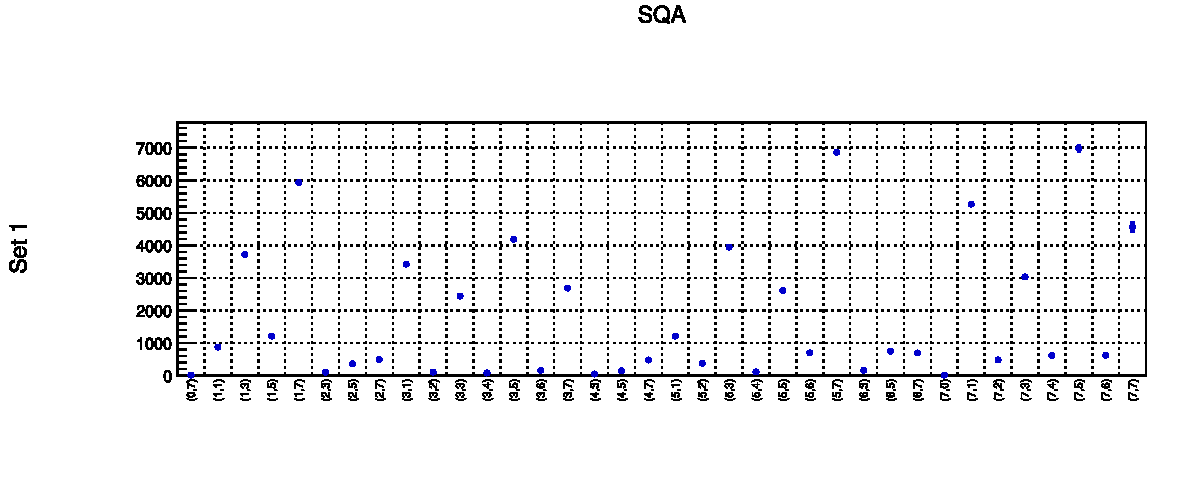
\includegraphics[width=1.08\linewidth]{Pictures/1}
			\end{subfigure}
			\hspace{-.73cm}
			\begin{subfigure}{.49\linewidth}
				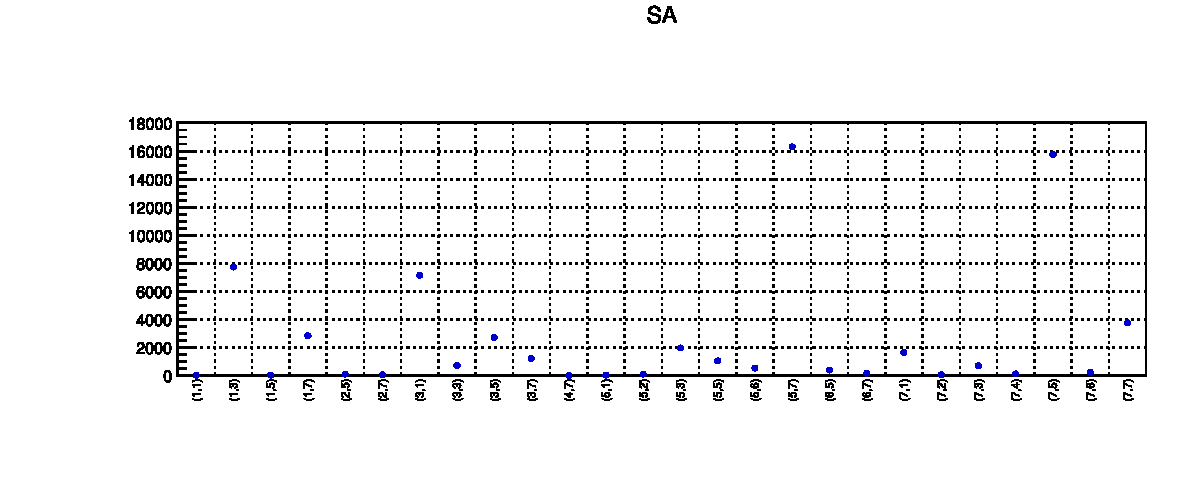
\includegraphics[width=1.08\linewidth]{Pictures/2}
			\end{subfigure}
			
			\vspace{-1.8cm}
			\begin{subfigure}{.49\linewidth}
				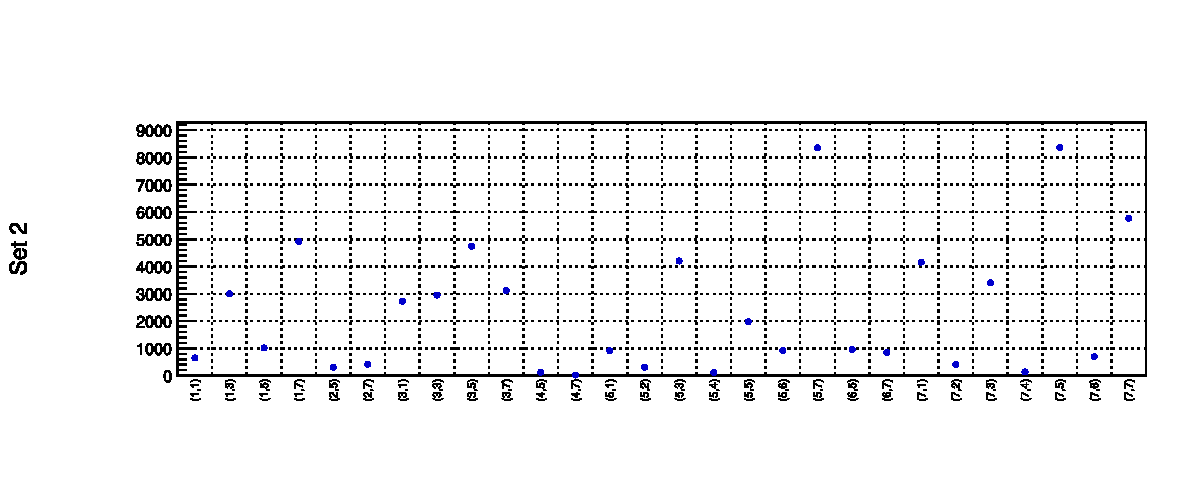
\includegraphics[width=1.08\linewidth]{Pictures/3}
			\end{subfigure}
			\hspace{-.73cm}
			\begin{subfigure}{.49\linewidth}
				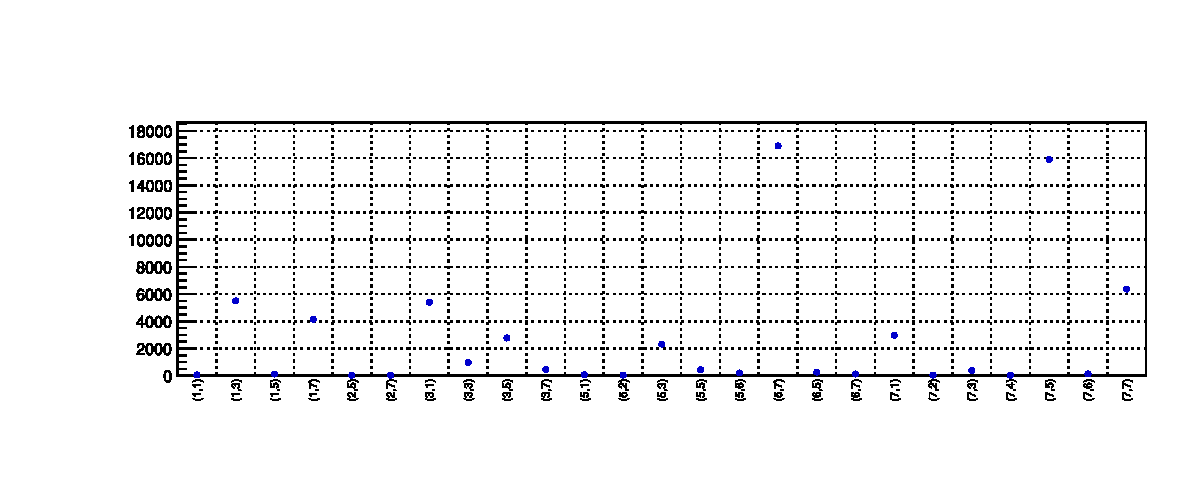
\includegraphics[width=1.08\linewidth]{Pictures/4}
			\end{subfigure}
			
			\vspace{-1.8cm}
			\begin{subfigure}{.49\linewidth}
				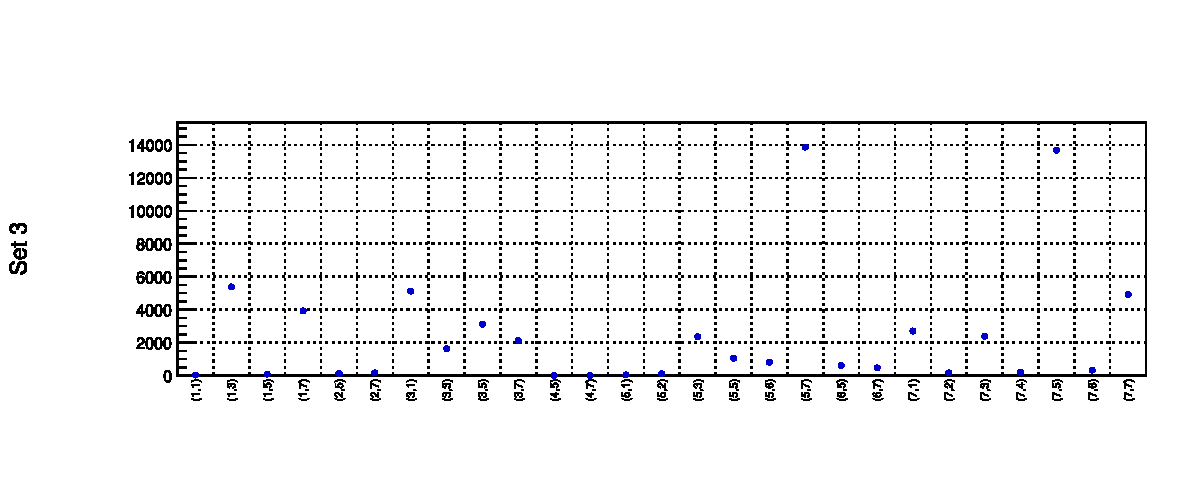
\includegraphics[width=1.08\linewidth]{Pictures/5}
			\end{subfigure}
			\hspace{-.73cm}
			\begin{subfigure}{.49\linewidth}
				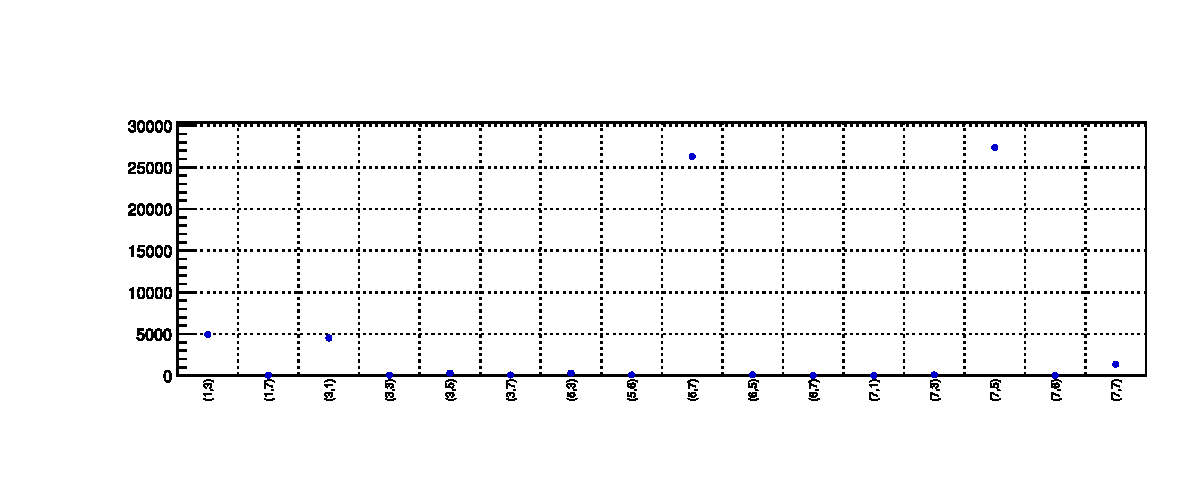
\includegraphics[width=1.08\linewidth]{Pictures/6}
			\end{subfigure}
			
			\vspace{-1.8cm}
			\begin{subfigure}{.49\linewidth}
				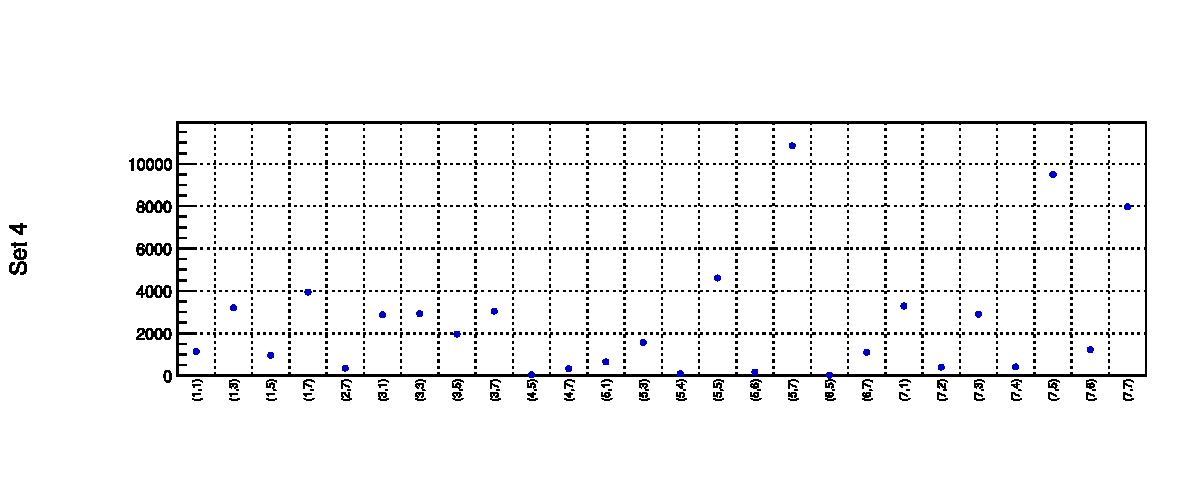
\includegraphics[width=1.08\linewidth]{Pictures/7}
			\end{subfigure}
			\hspace{-.73cm}
			\begin{subfigure}{.49\linewidth}
				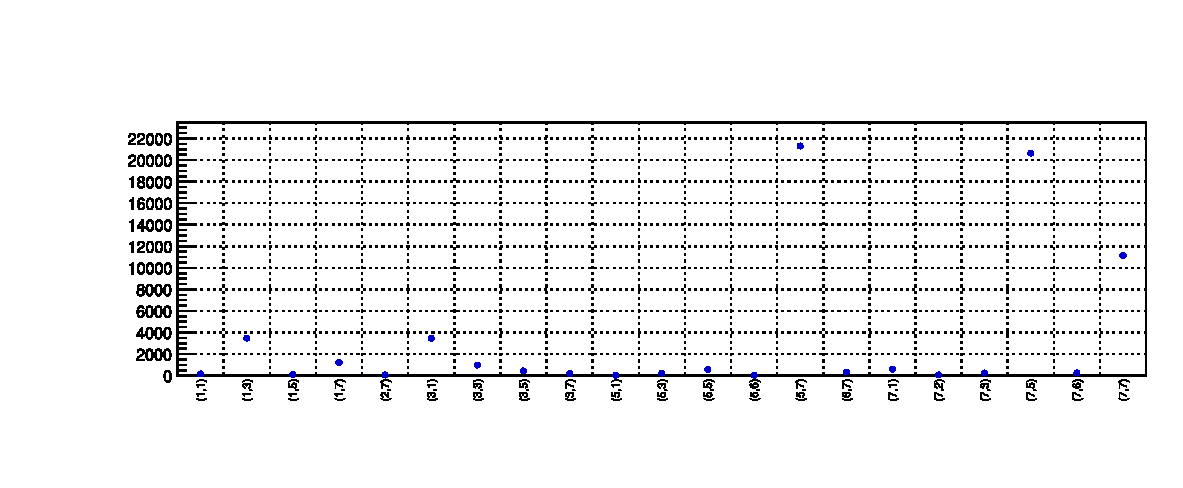
\includegraphics[width=1.08\linewidth]{Pictures/8}
			\end{subfigure}
			\caption{La Figura si legge come una tabella, sulle righe ci sono i diversi set di porte utilizzate, sulle colonne i diversi metodi di risoluzione; sull'asse $x$ di ogni grafico leggiamo gli assegnamenti di $A$ e $B$ osservati; sull'asse $y$ il numero medio di osservazioni per un certo assegnamento, l'errore associato alla misura è la deviazione standard.}
			\label{fig:fact}
		\end{figure}
		
		\par
	\end{landscape}
	\restoregeometry
}
	
	\section{Analisi della dimensione del QUBO}
	Per studiare come aumenta la dimensione del problema in funzione della dimensione dei fattori bisogna prima studiare la dimensione del circuito sintetizzato. In questa prima analisi non studiamo il circuito dal punto di vista dell'ingegneria elettronica, ci limitiamo invece a osservare quanto abbiamo prodotto attraverso Yosys. 
	
	\label{sec:dim}
	\begin{wrapfigure}{r}{.6\linewidth}
		\centering
		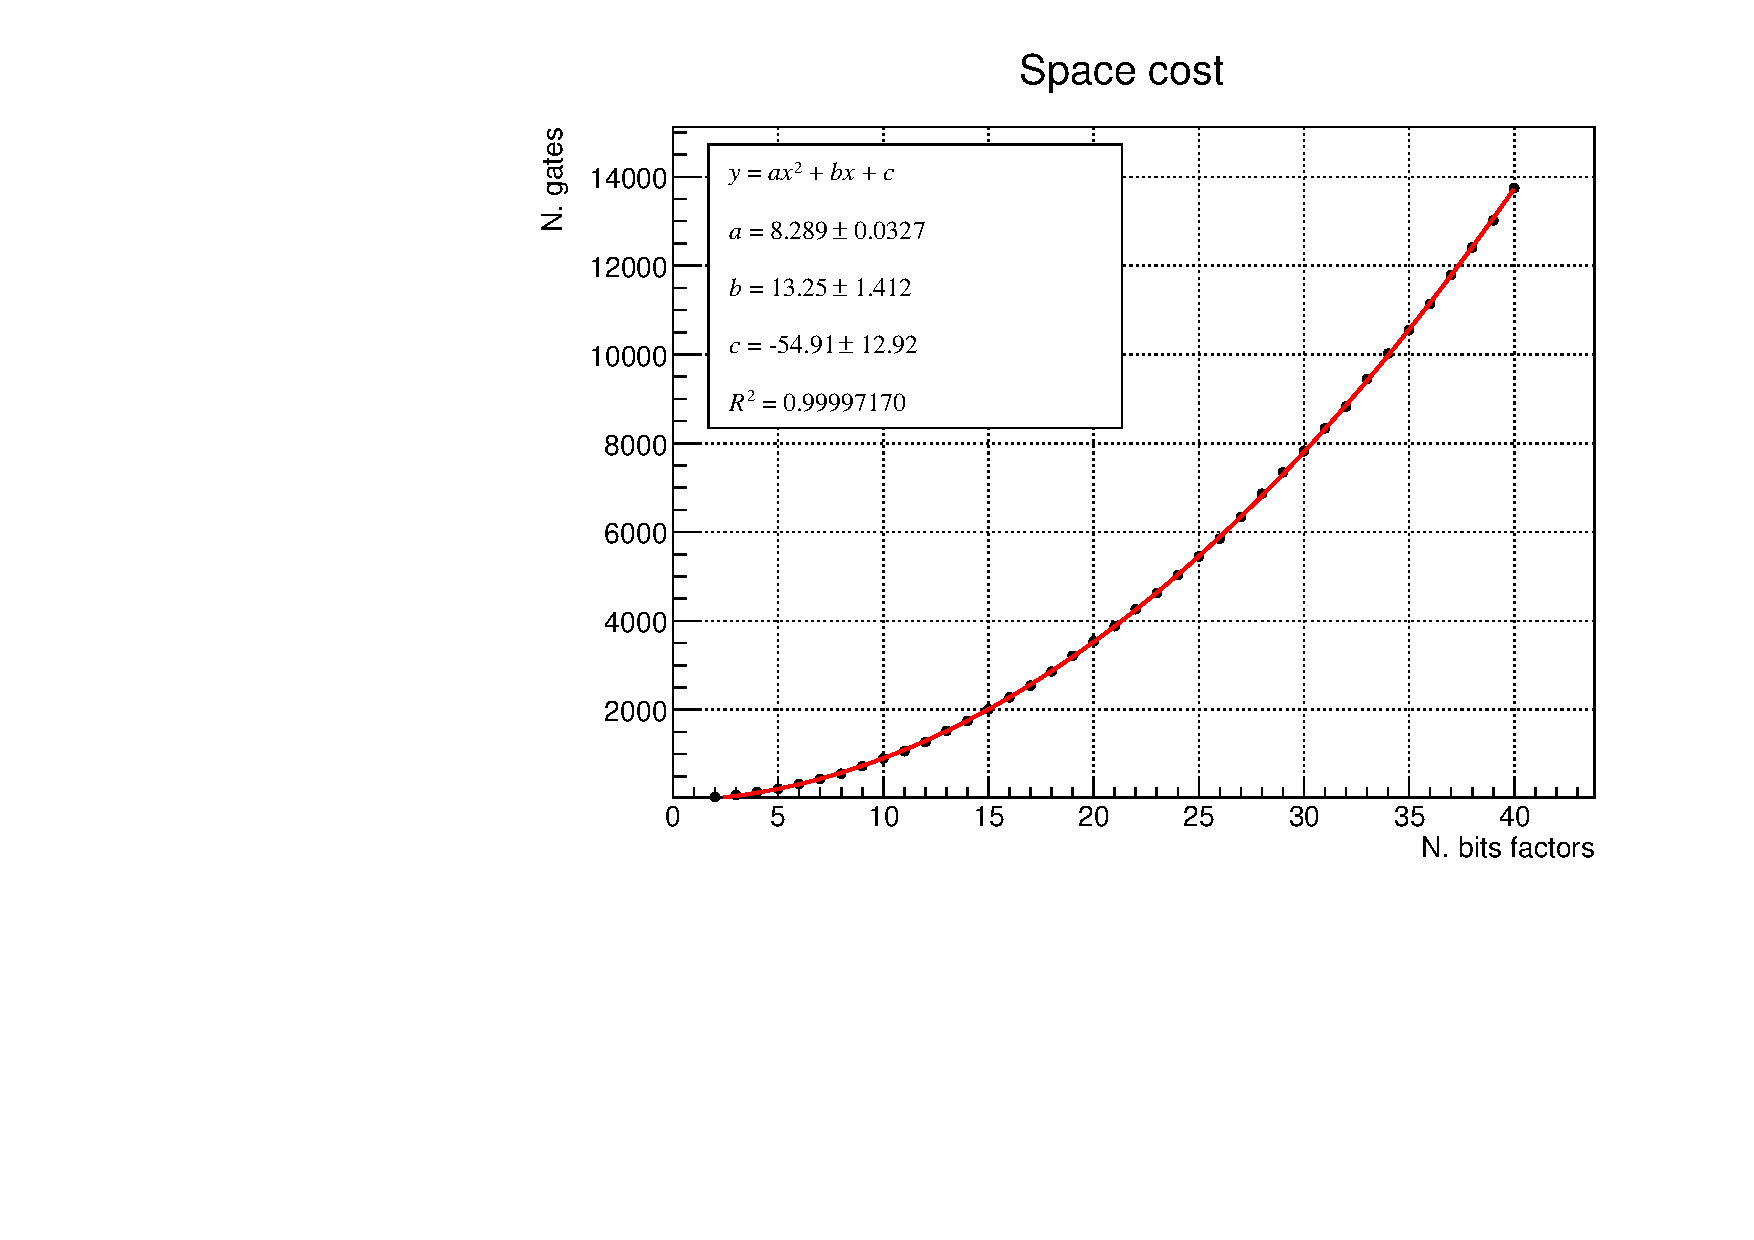
\includegraphics[width=\linewidth]{Pictures/dim}
		\caption{Gates in funzione dei bits dei fattori $A$ e $B$}
		\label{fig:dim}
	\end{wrapfigure}
	In  particolare a partire dal template del Listato \ref{lst:mult_verilog} e usando la Formula \ref{eqn:bits} per dimensionare il risultato generiamo via via circuiti che accenttano in input numeri sempre più grandi. Nell'Immagine \ref{fig:dim} si vede come aumenta il numero di gates in funzione del numero di bit dedicati a ciascun fattore della moltiplicazione. Il valore di $R^2$ molto vicino a $1$ suggerisce che la crescita quadratica ipotizzata descriva bene l'aumentare del numero di gates del circuito. 
	
	Dato che per ogni gate fa aumentare di un valore costante il numero di qubits necessari a rappresentare il problema Ising possiamo concludere che anche la dimensione del problema finale aumenta quadraticamente rispetto alle dimensioni dell'input.
	
	Questo è un risultato importante perchè se la dimensione del circuito crescesse esponenzialmente rispetto alla dimensione dell'input passeremmo da un problema che si risolve classicamente in tempo esponenziale a un problema che richiede spazio esponenziale, di fatto mettendoci in una situazione peggiore.
	\subsection{E Shor?}
	Da quello che ho trovato l'aricolo più recente è del 2024 \cite{bibid} e detto $N$ il valore da fattorizzare, con $n = \log_2 N$ il numero di qubit richiesti per implementare l'aloritmo di Shor è $\frac{n}{2} + o(n)$ con un numero di gates che è dell'ordine di $O(n^3)$ per una profondità di circuito che è $n^2 \log^3n$ e va eseguito più volte (l'articolo stima che per fattorizzare una chiave RSA a $2048$ bit servano $1730$ qubit logici e il circuito debba essere eseguito $40$ volte). 
	
	Questo risultato è interessante, infatti nonostante il numero di qubit logici richiesto dall'algoritmo di Shor sia infariore, il circuito quantistico da costruire cresce più rapidamente di quanto aumentino le dimensioni del problema Ising, questo significa anche più errori introdotti e un numero maggiore di qubit fisici per compensare la poca affidabilità dei gates quantistici. Questo non significa che questo approccio sia più efficiente dell'algoritmo di Shor, ma vuol anche dire che non va scartato aprescindere solo perchè il numero di qubits chresce quadraticamente.
	
	\section{Limitazioni e spunti}
	\label{sec:limit}
	È necessario studiare un po' di elettronica per capoire come descrivere un moltiplicatore, Yosys fa un ottimo lavoro, ma quando il numero di gates aumenta molto l'ottimizzazione inizia a richiedere veramente molto tempo.
	
	QAOA non testato si possono usare altri metodi oltre a \texttt{statevector}
	
	La dimensione dell'output va bene se si parte dall'input, al contrario non funziona più molto bene ade esempio...
	
\end{document}
